\documentclass[border=2pt]{standalone}
\usepackage{amsmath}
\usepackage{pgfplots}
\usepgfplotslibrary{groupplots}
\usetikzlibrary{calc}
\pgfplotsset{compat=1.18}
\begin{document}
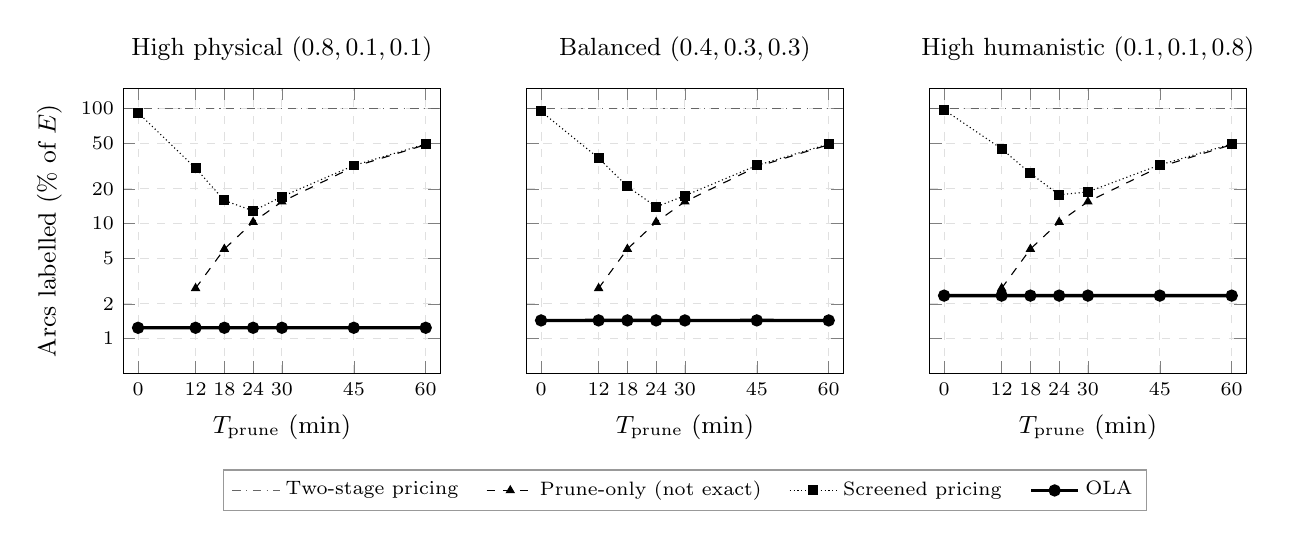
\begin{tikzpicture}
\begin{groupplot}[group style={group size=3 by 1, horizontal sep=1.1cm, y descriptions at=edge left},
  width=5.6cm, height=5.2cm, ymode=log, ymin=0.5, ymax=150,
  xmin=-3, xmax=63, xtick={0,12,18,24,30,45,60},
  xlabel={$T_{\text{prune}}$ (min)}, tick label style={font=\scriptsize}, label style={font=\small},
  title style={font=\small}, grid=major, grid style={dashed, black!12},
  ytick={1,2,5,10,20,50,100}, yticklabels={1,2,5,10,20,50,100}]
\nextgroupplot[title={High physical $(0.8,0.1,0.1)$}, ylabel={Arcs labelled (\% of $E$)}]
\addplot[black!60, thin, dashdotted, domain=-3:63, samples=2] {100};
\addplot[black, dashed, mark=triangle*, mark options={solid}, mark size=1.6pt] coordinates {(12,2.732) (18,5.990) (24,10.282) (30,15.465) (45,31.085) (60,48.400)};
\addplot[black, densely dotted, mark=square*, mark options={solid}, mark size=1.6pt] coordinates {(0,91.913) (12,30.227) (18,15.855) (24,12.845) (30,17.102) (45,31.913) (60,49.042)};
\addplot[black, solid, very thick, mark=*, mark size=1.6pt] coordinates {(0,1.238) (12,1.239) (18,1.239) (24,1.239) (30,1.239) (45,1.239) (60,1.239)};
\nextgroupplot[title={Balanced $(0.4,0.3,0.3)$}]
\addplot[black!60, thin, dashdotted, domain=-3:63, samples=2] {100};
\addplot[black, dashed, mark=triangle*, mark options={solid}, mark size=1.6pt] coordinates {(12,2.732) (18,5.990) (24,10.282) (30,15.465) (45,31.085) (60,48.400)};
\addplot[black, densely dotted, mark=square*, mark options={solid}, mark size=1.6pt] coordinates {(0,94.224) (12,36.988) (18,20.986) (24,13.929) (30,17.429) (45,31.942) (60,49.046)};
\addplot[black, solid, very thick, mark=*, mark size=1.6pt] coordinates {(0,1.435) (12,1.436) (18,1.436) (24,1.436) (30,1.435) (45,1.436) (60,1.435)};
\nextgroupplot[title={High humanistic $(0.1,0.1,0.8)$}, legend to name=grouplegend, legend columns=4, legend style={font=\scriptsize, draw=black!40, /tikz/every even column/.append style={column sep=8pt}}]
\addplot[black!60, thin, dashdotted, domain=-3:63, samples=2] {100};
\addlegendentry{Two-stage pricing}
\addplot[black, dashed, mark=triangle*, mark options={solid}, mark size=1.6pt] coordinates {(12,2.732) (18,5.990) (24,10.282) (30,15.465) (45,31.085) (60,48.400)};
\addlegendentry{Prune-only (not exact)}
\addplot[black, densely dotted, mark=square*, mark options={solid}, mark size=1.6pt] coordinates {(0,97.167) (12,44.577) (18,27.240) (24,17.738) (30,18.826) (45,32.289) (60,49.125)};
\addlegendentry{Screened pricing}
\addplot[black, solid, very thick, mark=*, mark size=1.6pt] coordinates {(0,2.358) (12,2.359) (18,2.358) (24,2.359) (30,2.359) (45,2.359) (60,2.358)};
\addlegendentry{OLA}
\end{groupplot}
\node[anchor=north] at ($(group c2r1.south)+(0,-1.1cm)$) {\pgfplotslegendfromname{grouplegend}};
\end{tikzpicture}
\end{document}
